% IEEE conference-style paper. Compile on Overleaf (IEEEtran is built in) or with pdflatex + bibtex-free (thebibliography).
% Every \res{...} marks a number to fill from results/report/summary.csv after the Kaggle runs.
\documentclass[conference]{IEEEtran}
\usepackage[T1]{fontenc}
\usepackage[utf8]{inputenc}
\usepackage{graphicx,booktabs,multirow,amsmath,xcolor,url,hyperref}
\hypersetup{hidelinks}
\usepackage{algorithm,algpseudocode}
\usepackage{tikz}
\usetikzlibrary{positioning,arrows.meta}
\graphicspath{{figures/}{../results/report/}}
\newcommand{\res}[1]{\textcolor{red}{[#1]}}
\newcommand{\sys}{\textsc{sensor-LST}}

\begin{document}
\title{Update-Heavy Workloads on Small Clusters: An Experimental Comparison of Delta Lake, Apache Iceberg and Apache Hudi for IoT and Hydro-Meteorological Data}

\author{\IEEEauthorblockN{H\`a V\u{a}n Vinh, \DJ{}\~{\^o} Th\d{i} Lan}
\IEEEauthorblockA{Big Data Analytics and Management (TLU 2026), Hanoi, Vietnam}}

\maketitle

\begin{abstract}
Lakehouse table formats---Delta Lake, Apache Iceberg and Apache Hudi---add ACID transactions, schema evolution and
time travel on top of open file formats, but published comparisons (LHBench, LST-Bench) mostly run read-heavy TPC-DS
on large cloud clusters. Monitoring systems for rainfall, water level and water quality behave differently: data
arrive continuously in micro-batches, late readings must be corrected retroactively, and whole station-days are
occasionally deleted. We present \sys{}, an open-source workload generator built on the TSM-Bench d1 hydrological
dataset that replays appends, late-data upserts and station-level deletes, with a ground-truth checksum at every
checkpoint. We evaluate the three formats in copy-on-write and merge-on-read modes (Delta: deletion vectors),
four late-update rates $u\in\{0,1,5,20\}\%$ and three compaction cadences on a single 4-vCPU node, 380 runs in
total, all of which match the ground truth. Any late data at all raises total cost 1.3--3.8$\times$ over append-only
ingestion, but the cost is nearly flat between $u=1\%$ and $u=20\%$ ($\le$8\% spread): scattered corrections touch
every file of the recent partitions regardless of their number. Iceberg merge-on-read is the cheapest layout for every
$u>0$, 2.7--4.4$\times$ cheaper than Delta or Hudi without compaction, with write amplification 1.0--1.2 against
9.4--11 for copy-on-write; compacting every 20 batches returns reads to near copy-on-write latency for 8\,s of extra work, although latency climbs again between compactions.
Delta's deletion vectors cut bytes written eightfold yet were slower than Delta copy-on-write in both ingest and reads
at this scale. Metadata grows linearly by 11--72\,KB per batch, and Hudi keeps only 23 versions reachable by time
travel. We distil the results into a decision table for small water-monitoring deployments and release all code,
configurations and raw measurements.
\end{abstract}

\begin{IEEEkeywords}
Lakehouse, Delta Lake, Apache Iceberg, Apache Hudi, copy-on-write, merge-on-read, compaction, time travel,
benchmarking, time series
\end{IEEEkeywords}

%=====================================================================================================
\section{Introduction}
The lakehouse architecture~\cite{armbrust2021lakehouse} stores tables as open columnar files on cheap storage
and recovers warehouse features---transactions, versioning, data skipping---through a metadata layer. Three such
\emph{log-structured table} (LST) formats dominate: Delta Lake~\cite{armbrust2020delta}, Apache
Iceberg~\cite{iceberg-spec} and Apache Hudi~\cite{hudi-docs}. Research has moved from \emph{whether} to adopt them
to the \emph{design trade-offs} between them: how row-level changes are written, how metadata is organised and how
small files are compacted~\cite{jain2023lhbench,camacho2024lstbench,gruenheid2025autocomp}.

\textbf{Monitoring data are update-heavy.} Hydro-meteorological networks produce wide sensor tables
(one row per station and timestamp, one column per sensor). Readings arrive every few minutes; delayed or
corrected readings arrive hours later and must overwrite earlier values; a faulty station's data are deleted for a
whole day. The resulting workload is dominated by small appends, keyed upserts into recent partitions and
selective deletes---not by the large scans of TPC-DS.

\textbf{Small clusters are the norm.} Provincial agencies and universities in Vietnam typically run analytics on one
to four commodity servers, not on elastic cloud clusters. Existing comparisons were executed on cloud clusters with
TPC-DS at 1--3\,TB~\cite{jain2023lhbench,camacho2024lstbench}; it is unclear whether their conclusions hold for
update-heavy workloads at a scale of gigabytes on one node.

\textbf{Research questions.}
\begin{itemize}
\item \textbf{RQ1:} For late-update rates $u\in\{0,1,5,20\}\%$, which format and write mode yield the lowest total
cost (ingest + compaction + queries)?
\item \textbf{RQ2:} Which compaction cadence best balances the number of small files against read latency?
\item \textbf{RQ3:} How does metadata grow with the number of commits, and how does it affect time travel?
\end{itemize}
Before running the experiments we stated three hypotheses, derived from LHBench and LST-Bench:
\textbf{H1}---at low update rates the formats differ mainly on the read path, as LHBench found for TPC-DS;
\textbf{H2}---at high update rates merge-on-read lowers write cost but raises read latency until compaction;
\textbf{H3}---there is a break point in the number of small files beyond which periodic compaction clearly pays off.

\textbf{Summary of findings.} H1 does not hold for this workload: at gigabyte scale the formats differ mainly on the
\emph{write} path and in fixed per-operation overheads. H2 holds for Iceberg and Hudi but not for Delta Lake, whose
deletion vectors saved bytes but not time. H3 holds in a weak form: read latency of merge-on-read tables starts to climb
after about 20 batches; compacting at that cadence recovers copy-on-write read speed cheaply, but only until delete files accumulate again. In addition:
\begin{itemize}
\item the \emph{presence} of late data, not its rate, determines cost (a 1.3--3.8$\times$ step from 0\% to 1\%, then
$\le$8\% change up to 20\%);
\item Iceberg merge-on-read was the cheapest layout for every non-zero update rate;
\item ingest latency did not grow with table size over the run, because partition pruning bounds each MERGE to the
most recent four days;
\item several defaults and corner cases change results or correctness: Hudi's timestamp record keys, Hudi's compaction
trigger and timeline archiving, Iceberg's dangling delete files after compaction, and Delta's synchronous log
checkpoints.
\end{itemize}

\textbf{Organisation.} Section~\ref{sec:bg} reviews the three formats and related benchmarks;
Section~\ref{sec:workload} describes \sys{}; Section~\ref{sec:setup} the experimental setup;
Section~\ref{sec:results} the results for RQ1--RQ3, a breakdown by operation, query and time, an ablation and a statistical check;
Section~\ref{sec:disc} explains the results, lists practical pitfalls and gives a decision table;
Section~\ref{sec:concl} concludes.

\textbf{Contributions.} (1)~\sys{}, an open workload generator that turns TSM-Bench~\cite{khelifati2023tsmbench}
data into a deterministic stream of appends, late upserts and deletes, with ground truth for correctness checking;
(2)~a controlled, reproducible comparison of Delta Lake, Iceberg and Hudi (plus a plain-Parquet baseline) in both
write modes and three compaction cadences on a single node, 380 runs with repetitions and randomised
interleaving; (3)~an explanation of the observed differences in terms of each format's write path, and a decision
table for practitioners.

%=====================================================================================================
\section{Background and Related Work}\label{sec:bg}
\subsection{Log-structured table formats}
All three formats store data as immutable Parquet files and keep a separate, versioned description of which files
form the table at each point in time. Because data files are never modified in place, every change produces new files
plus a new table version, much like the runs of a log-structured merge tree~\cite{oneil1996lsm}; this is why
Camacho-Rodr\'iguez et al.\ call them log-structured tables~\cite{camacho2024lstbench}. Table~\ref{tab:design}
summarises the design choices that matter for our workload.

\emph{Delta Lake} records each commit as a JSON file of actions (\texttt{add}, \texttt{remove}, \texttt{metaData},
\dots) in an ordered transaction log, \texttt{\_delta\_log}~\cite{armbrust2020delta}. A writer commits by atomically
creating the next numbered log file; readers reconstruct the current snapshot by replaying the log from the latest
Parquet \emph{checkpoint}, which by default is written every 10 commits. File-level statistics (min/max per column)
are stored in the \texttt{add} actions and drive data skipping.

\emph{Apache Iceberg} keeps a tree of metadata per snapshot~\cite{iceberg-spec}: a table metadata JSON points to the
current snapshot's \emph{manifest list}, which points to Avro \emph{manifests}, which list data files and delete files
with partition values and column statistics. A commit writes new manifests and a new metadata JSON and then swaps the
catalog pointer atomically. Query planning reads only the manifests whose partition ranges match the filter.

\emph{Apache Hudi} organises a table into \emph{file groups}, each identified by a file ID and consisting of
successive \emph{file slices}: a base Parquet file and, in merge-on-read tables, row-based log files with later
changes~\cite{hudi-docs}. A \emph{timeline} of instants (requested, inflight, completed) records every commit,
compaction and clustering action, and an internal metadata table caches file listings. Every record carries a key; a
key index (Bloom filters by default) routes upserts to the file group that holds the key, and \emph{small-file
handling} routes inserts into existing file groups below a size threshold so that files grow towards their target size.
Completed instants beyond a window are \emph{archived} out of the active timeline.

\begin{table}[t]
\centering\caption{Design choices relevant to update-heavy ingestion}\label{tab:design}
\footnotesize
\begin{tabular}{@{}p{1.55cm}p{1.95cm}p{1.95cm}p{1.95cm}@{}}\toprule
 & Delta Lake & Iceberg & Hudi\\\midrule
Version log & JSON commit files + Parquet checkpoint every 10 & metadata JSON $\rightarrow$ manifest list $\rightarrow$ manifests & timeline of instants + metadata table\\
Row-level change (MoR) & deletion-vector bitmap per file & position-delete files & log files per file group\\
Record keys & none (join on predicate) & none (join on predicate) & mandatory; key index\\
File sizing on write & none & target size & small-file handling\\
Time-travel horizon (defaults) & until \texttt{VACUUM} & until snapshot expiry & active timeline only\\\bottomrule
\end{tabular}
\end{table}

\textbf{Row-level changes.} Under \emph{copy-on-write} (CoW) every file containing a changed row is rewritten.
\emph{Merge-on-read} (MoR) instead records the change cheaply and reconciles it at read time: Iceberg v2 writes
position-delete files plus new data files~\cite{iceberg-spec}; Hudi appends changed records to log files of the
affected file group~\cite{hudi-docs}; Delta Lake has no log-file MoR, but \emph{deletion vectors} mark removed rows of
an existing file in a bitmap, so UPDATE and MERGE write only the new row versions~\cite{delta-dv}. We therefore
treat deletion vectors as Delta's MoR mode, and make the difference explicit in our analysis.

\textbf{Compaction.} Frequent small commits create small files and, under MoR, accumulate delete/log files.
Each format offers a maintenance operation: Delta \texttt{OPTIMIZE} (and \texttt{REORG \dots APPLY (PURGE)} to
materialise deletion vectors), Iceberg \texttt{rewrite\_data\_files}, and Hudi compaction (MoR) or clustering (CoW).

\subsection{Benchmarks}
Jain et al.~\cite{jain2023lhbench} analyse the design of the three formats and publish LHBench: on TPC-DS at 3\,TB,
performance differences are explained mostly by data read time, and Hudi loads more slowly because it is optimised for
keyed upserts. LST-Bench~\cite{camacho2024lstbench} extends TPC-DS with workload patterns (data maintenance,
optimisation, time travel) and metrics for performance stability across sessions. AutoComp~\cite{gruenheid2025autocomp}
reports LinkedIn's experience that small-file proliferation is a first-order operational problem and proposes
automated compaction. Harby and Zulkernine~\cite{harby2025survey} survey data lake, warehouse and lakehouse systems.
TSM-Bench~\cite{khelifati2023tsmbench} benchmarks seven time-series databases with queries derived from a water
monitoring use case; we reuse its dataset, not its systems. TPC-DS~\cite{nambiar2006tpcds} remains the reference
analytical workload. To our knowledge no published study combines update-heavy sensor workloads, both write modes,
controlled compaction cadence and single-node hardware.

\begin{table}[!t]\centering
\caption{Comparison with related benchmarks}\label{tab:related}
\footnotesize\setlength{\tabcolsep}{3pt}
\begin{tabular}{@{}p{1.75cm}p{2.15cm}p{1.75cm}p{2.5cm}@{}}\toprule
Study & Workload & Scale & Main focus\\\midrule
LHBench~\cite{jain2023lhbench} & TPC-DS, merge & 3\,TB, cluster & design trade-offs of three formats\\
LST-Bench~\cite{camacho2024lstbench} & TPC-DS, maintenance & cloud cluster & stability under maintenance\\
AutoComp~\cite{gruenheid2025autocomp} & production tables & data-lake scale & automated compaction\\
TSM-Bench~\cite{khelifati2023tsmbench} & monitoring queries & time-series DBs & TSDB ingestion and queries\\
This work & sensor appends, late upserts, deletes & 222\,MB, 1 node, 4 vCPU & update rate and compaction cadence on small hardware\\\bottomrule
\end{tabular}
\end{table}

\subsection{Time-series data and monitoring}
Time-series management systems are surveyed by Jensen et al.~\cite{jensen2017tsms}; specialised time-series databases
optimise ingestion of append-mostly streams and time-range queries. TSM-Bench~\cite{khelifati2023tsmbench} evaluates
such systems on monitoring workloads and found that no single system dominates across ingestion and query types.
Lakehouse formats target a different point: they store the same data as open files that any engine can read, and they
add versioning, which monitoring agencies need for audit and for recomputing results after corrections. Our workload
keeps TSM-Bench's data and query style but adds the late corrections and deletions that real monitoring networks see.

\subsection{Benchmark methodology}
Performance on shared cloud machines varies over time and between instances of the same type, which threatens the
repeatability of cloud benchmarks~\cite{leitner2016chaos,uta2020reproducible}. We follow the usual remedies: repeated
runs, randomised interleaving of the compared systems on the same machine, reporting of dispersion, and an explicit
calibration configuration to quantify machine-to-machine differences (Section~\ref{sec:setup}).

%=====================================================================================================
\section{The \sys{} Workload}\label{sec:workload}
\subsection{Design goals}
\sys{} is built to make the comparison fair and checkable: (i)~every format must receive byte-identical input, so the
generator materialises the whole operation stream before any run; (ii)~the workload must be deterministic given a seed,
so that runs on different machines are comparable; (iii)~every run must be verifiable, so the generator also computes
the expected table state; and (iv)~the parameters that drive the trade-offs studied here---late-update rate, delete
frequency, compaction cadence---must be explicit and independent.

\subsection{Data}
TSM-Bench d1 contains 10 stations $\times$ 100 sensors sampled every 10\,s for 60 days (5.18\,M rows), generated from
water temperature and level series of the Swiss Federal Office for the Environment~\cite{khelifati2023tsmbench}.
We keep its wide schema \texttt{(time, id\_station, s0..sK)} and add \texttt{day} (partition column) and
\texttt{ingest\_batch}. The main scale (\emph{small}) uses 10 stations $\times$ 20 sensors $\times$ 17 days
(1.47\,M rows, 253\,MB as Parquet). We observed that the d1 values are normalised and close to uniform on $[0,1)$
with little autocorrelation; they compress poorly, which raises absolute byte counts but affects all formats
equally.

\subsection{Operation stream}
The generator stages every operation as Parquet before any run, so all formats ingest byte-identical input:
\begin{enumerate}
\item \textbf{Bulk load} of 7 days of history (604{,}800 rows).
\item \textbf{40 micro-batches}, each covering 6\,h of event time (21{,}600 new rows). For $u>0$ the batch also
carries $\lfloor u\cdot 21{,}600\rceil$ late corrections: distinct, existing keys drawn uniformly from the preceding
72\,h, with new values. Batches are written with \emph{append} when $u=0$ and \emph{upsert} (MERGE) otherwise.
\item \textbf{GDPR-style delete} of one station-day every 10 batches.
\item \textbf{Compaction} every $k\in\{\infty,5,20\}$ batches.
\item \textbf{Checkpoint} every 10 batches: five queries, time travel and storage statistics.
\end{enumerate}
The generator maintains the expected table state and records the row count and $\sum s_0$ after each checkpoint; every
run is checked against this ground truth. Algorithm~\ref{alg:gen} gives the procedure and Table~\ref{tab:params} the
parameters of the \emph{small} scale used in all experiments.

\begin{algorithm}[t]
\caption{\sys{} stream generation for late-update rate $u$}\label{alg:gen}
\begin{algorithmic}[1]
\State $S \gets$ source rows with $t < t_0 + H$ \Comment{history, bulk-loaded}
\State write $S$ as \texttt{base}; $E \gets \{(k, s_0(k)) : k \in S\}$ \Comment{expected state}
\For{$i = 1 \dots B$}
  \State $N \gets$ source rows with $t \in [t_0{+}H{+}(i{-}1)\Delta,\; t_0{+}H{+}i\Delta)$
  \State $L \gets$ sample $\lfloor u\,|N|\rceil$ distinct keys of $E$ with $t \ge$ batch start $- W$
  \State give every row of $L$ new random sensor values
  \State write $N \cup L$ as \texttt{batch}$_i$; update $E$ with $L$, then add $N$
  \If{$i \bmod D = 0$} \State choose station $s$ and day $d$; record \textsc{delete}$(s,d)$; remove them from $E$ \EndIf
  \If{$i \bmod C = 0$} \State record checkpoint $(|E|, \sum_{k\in E} s_0(k))$ \EndIf
\EndFor
\end{algorithmic}
\end{algorithm}

\begin{table}[t]\centering
\caption{Workload parameters (\emph{small} scale)}\label{tab:params}
\footnotesize
\begin{tabular}{@{}lll@{}}\toprule
Parameter & Symbol & Value\\\midrule
Stations $\times$ sensors & -- & 10 $\times$ 20 (TSM-Bench d1)\\
Sampling interval & -- & 10\,s\\
History (bulk load) & $H$ & 7 days, 604{,}800 rows\\
Micro-batches & $B$ & 40 $\times$ 6\,h = 10 days\\
New rows per batch & $|N|$ & 21{,}600\\
Late-update rate & $u$ & 0, 1, 5, 20\% (0--4{,}320 rows)\\
Late window & $W$ & 72\,h\\
Delete every & $D$ & 10 batches (one station-day)\\
Checkpoint every & $C$ & 10 batches\\
Compaction every & $k$ & never, 5, 20 batches\\
Final table & -- & 1.43\,M rows, $\approx$222\,MB Parquet\\\bottomrule
\end{tabular}
\end{table}

\subsection{Queries}
Q1 computes hourly averages per station over the last 24\,h; Q2 the top-5 stations by peak value over 72\,h;
Q3 a daily regional average via a join with station metadata over all history; Q4 a 2-hour range of one sensor at one
station; Q5 a full scan (\texttt{count}, $\sum s_0$) that doubles as the checksum. Each query runs twice per checkpoint
(cold, warm). Time travel reads the version 5 commits before the latest and the first version.

%=====================================================================================================
\section{Experimental Setup}\label{sec:setup}
\textbf{Platform.} Kaggle CPU notebooks (4 vCPU, 31.3\,GB RAM, Linux 6.18, local disk), run as headless batch
jobs. Each update rate ran in two batches, repetitions 1--3 and repetitions 4--5, each on its own VM (eight VMs in total). The calibration
configuration (Delta CoW, $u=0$) took 65, 103, 70 and 98\,s on the first-batch VMs of the $u=0,1,5,20\%$ shards and 98, 86, 100 and
99\,s on the second-batch VMs, i.e.\ six of the eight VMs were 1.3--1.6$\times$ slower than the reference.
Comparisons between formats are always made within one VM; for comparisons across update rates we divide every
duration by its VM's calibration factor (first batch 1.00, 1.58, 1.07, 1.50; second batch 1.51, 1.32, 1.54, 1.51), expressing all times in seconds of the
$u=0$ VM. Apache Spark~\cite{zaharia2012rdd,armbrust2015sparksql}
3.5.3 runs in local mode with all cores, driver memory 60\% of RAM, Java 21 and Python 3.13 (the platform defaults; all four layouts were verified to give
identical results on Java 11/21 and Python 3.12/3.13), one fresh JVM per run.
Versions: Delta Lake 3.2.1, Iceberg 1.6.1 (Hadoop catalog, format v2), Hudi 0.15.0.

\textbf{Configurations} (Table~\ref{tab:config}). All formats write snappy Parquet (defaults differ: Iceberg zstd,
Hudi gzip), partition by \texttt{day}, and never clean old files during a run (no \texttt{VACUUM}, snapshot expiry or
Hudi cleaner), so bytes on disk equal bytes written and every version stays reachable. MERGE and DELETE statements
carry an explicit \texttt{day IN (\dots)} predicate. Hudi keys records on a derived string
\texttt{id\_station|epoch\_micros}: with a timestamp key field, its bulk-insert and upsert paths rendered the key
differently and silently duplicated records---an issue our checksum caught during development. Hudi compaction is
scheduled after every delta commit so that our cadence, not Hudi's default of five delta commits, controls it.
The plain-Parquet baseline rewrites the affected day partitions on every upsert or delete.
We keep each format's default timeline retention: Delta and Iceberg keep every version until an explicit
\texttt{VACUUM}/snapshot expiry, whereas Hudi archives completed instants beyond its active-timeline window
(\texttt{hoodie.keep.min/max.commits} = 20/30) even with the cleaner disabled, so only active instants remain
reachable by time travel. ``Versions'' below therefore means versions reachable by time travel.

\begin{table}[t]
\centering\caption{Write modes and maintenance operations per format}\label{tab:config}
\scriptsize\setlength{\tabcolsep}{3pt}
\begin{tabular}{@{}llll@{}}
\toprule
 & Delta Lake 3.2.1 & Iceberg 1.6.1 & Hudi 0.15.0\\ \midrule
CoW & rewrite files & \texttt{copy-on-write} & \texttt{COPY\_ON\_WRITE}\\
MoR & deletion vectors & position deletes & log files\\
Compact & \texttt{REORG}+\texttt{OPTIMIZE} & \texttt{rewrite\_data\_files} & compaction / clustering\\
\bottomrule
\end{tabular}
\end{table}

Table~\ref{tab:settings} lists the settings that differ from each system's defaults; everything else is left as shipped.

\begin{table}[!t]\centering
\caption{Non-default settings used in every run}\label{tab:settings}
\scriptsize\setlength{\tabcolsep}{3pt}
\begin{tabular}{@{}lp{6.5cm}@{}}\toprule
Scope & Setting\\\midrule
Spark & \texttt{spark.sql.shuffle.partitions} = 2 $\times$ cores; session time zone UTC; Parquet codec snappy\\
Delta & \texttt{enableDeletionVectors} on for MoR, off for CoW\\
Iceberg & \texttt{write.parquet.compression-codec} = snappy; \texttt{write.\{delete,update,merge\}.mode} = merge-on-read or copy-on-write\\
Hudi & \texttt{hoodie.parquet.compression.codec} = snappy; \texttt{hoodie.clean.automatic} = false; inline compaction and clustering off; \texttt{hoodie.compact.inline.max.delta.commits} = 1; record key \texttt{hkey}\\\bottomrule
\end{tabular}
\end{table}

\textbf{Experiment matrix.} 3 formats $\times$ 2 modes $\times$ 4 update rates $\times$ 3 compaction cadences = 72
configurations, plus 4 Parquet baselines, each repeated 5 times: 380 runs. Runs are executed in rounds (one
repetition of every configuration per round) in a seeded random order, so that formats are interleaved on the same
machine. Each update rate runs as a separate shard on its own VM; every shard also repeats a calibration
configuration (Delta CoW, $u=0$) to quantify VM-to-VM variation.

\textbf{Metrics.} Ingest time per operation; compaction time; warm and cold query latency; \emph{write amplification}
= bytes of data files written / bytes of the final logical table written once as snappy Parquet; live data files and
delete/log files; metadata bytes and files; number of versions; time-travel latency; \emph{degradation rate}
$(L_{last}-L_{first})/L_{first}$ of warm Q1--Q5 latency across checkpoints, in the spirit of
LST-Bench~\cite{camacho2024lstbench}. We report medians and the coefficient of variation (CV) over repetitions.

\textbf{Measurement procedure.} The runner times each operation with a monotonic clock around the Spark action that
completes it, so times include planning, execution and commit. After every operation it lists the table directory and
attributes each new or grown file to data or metadata (Hadoop's local \texttt{.crc} side files are ignored because they
do not exist on object storage); the sum over the run is the bytes written. Live files are read from each format's own
metadata (Delta: log replay, keyed on file and deletion vector; Iceberg: the \texttt{files} metadata table; Hudi: latest
file slice per file group minus groups replaced by clustering). At the end, the current table is written once as
plain snappy Parquet partitioned by day; its size is the denominator of write amplification. Each run writes one JSON
record with every operation, checkpoint and statistic; all analysis is computed from these records.
Fig.~\ref{fig:pipeline} shows the pipeline.

\begin{figure}[t]\centering
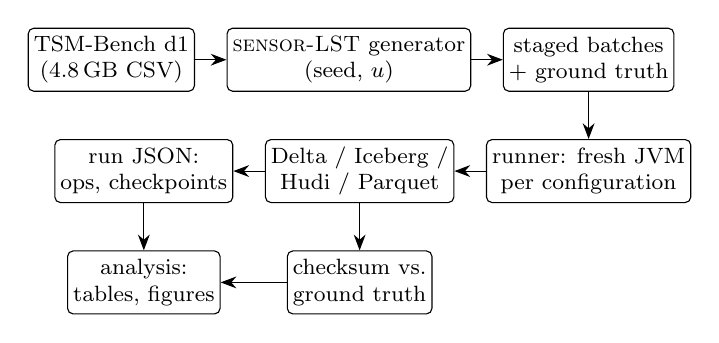
\begin{tikzpicture}[font=\footnotesize, node distance=3mm and 4mm,
  box/.style={draw, rounded corners=2pt, align=center, minimum height=8mm, inner sep=2pt},
  arr/.style={-{Stealth[length=2mm]}}]
\node[box] (d1) {TSM-Bench d1\\(4.8\,GB CSV)};
\node[box, right=of d1] (gen) {\sys{} generator\\(seed, $u$)};
\node[box, right=of gen] (stage) {staged batches\\+ ground truth};
\node[box, below=6mm of stage] (run) {runner: fresh JVM\\per configuration};
\node[box, left=of run] (fmt) {Delta / Iceberg /\\Hudi / Parquet};
\node[box, left=of fmt] (json) {run JSON:\\ops, checkpoints};
\node[box, below=6mm of fmt] (chk) {checksum vs.\\ground truth};
\node[box, below=6mm of json] (ana) {analysis:\\tables, figures};
\draw[arr] (d1) -- (gen); \draw[arr] (gen) -- (stage); \draw[arr] (stage) -- (run);
\draw[arr] (run) -- (fmt); \draw[arr] (fmt) -- (json); \draw[arr] (fmt) -- (chk);
\draw[arr] (json) -- (ana); \draw[arr] (chk) -- (ana);
\end{tikzpicture}
\caption{Experiment pipeline. The operation stream is generated once per update rate; every run replays it on one
layout in a fresh JVM and is checked against the ground truth at each checkpoint.}
\label{fig:pipeline}
\end{figure}

%=====================================================================================================
\section{Results}\label{sec:results}
\textbf{Correctness and stability.} All 395 runs (380 plus 15 calibration repeats) returned the expected row count and
checksum at all four checkpoints. The median coefficient of variation of total cost across the three repetitions is
3.6\% (maximum 10.9\%, Iceberg CoW at $u=20\%$), so differences above about 15\% are well outside run-to-run noise.
Fig.~\ref{fig:var} shows both sources of variation: repetitions on the same VM lie close together, whereas the same
calibration configuration took 65 to 103\,s on different VMs of the same advertised type---a 1.6$\times$ spread that
would have distorted every comparison across update rates without normalisation.

\begin{figure}[t]\centering
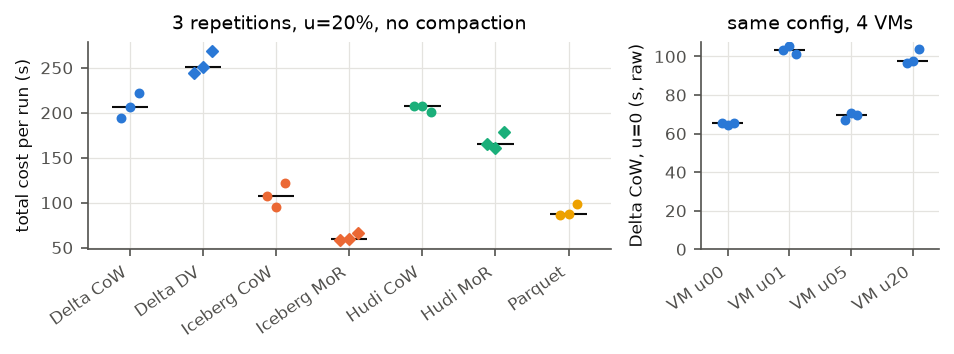
\includegraphics[width=\columnwidth]{fig_variability.png}
\caption{Run-to-run and machine-to-machine variation. Left: total cost of each repetition (bar = median). Right: the
calibration configuration on the four VMs, in raw seconds.}
\label{fig:var}
\end{figure}
Table~\ref{tab:u20} summarises the $u=20\%$ shard.

\begin{table*}[t]\centering
\caption{Results at $u=20\%$ (median of 5 runs, seconds on the reference VM). Total = ingest + compaction + all
checkpoint queries. WA = write amplification. Read = warm Q1--Q5 at the last checkpoint. Files = live data + live
delete/log files at the end.}\label{tab:u20}
\footnotesize
\begin{tabular}{@{}lrrrrrrrr@{}}\toprule
Layout & Compact every & Ingest & Compaction & Queries & Total & WA & Read & Files\\\midrule
Iceberg MoR & -- & 55 & 0 & 8 & \textbf{63} & 1.16 & 2.27 & 167+154\\
Parquet (rewrite) & -- & 89 & 0 & 3 & 92 & 9.53 & 0.70 & 84+0\\
Iceberg CoW & -- & 97 & 0 & 3 & 100 & 9.37 & 0.63 & 17+0\\
Hudi MoR & -- & 159 & 0 & 11 & 170 & 2.51 & 2.86 & 5+124\\
Hudi CoW & -- & 204 & 0 & 3 & 208 & 11.00 & 0.80 & 11+0\\
Delta CoW & -- & 215 & 0 & 7 & 223 & 9.37 & 1.64 & 17+0\\
Delta DV & -- & 236 & 0 & 19 & 256 & 1.16 & 4.76 & 167+154\\\midrule
Iceberg MoR & 20 & 52 & 8 & 4 & \textbf{64} & 2.34 & 0.67 & 17+10\\
Iceberg CoW & 20 & 96 & 0 & 3 & 99 & 9.37 & 0.71 & 17+0\\
Hudi MoR & 20 & 162 & 17 & 7 & 186 & 3.46 & 1.19 & 17+0\\
Delta CoW & 20 & 200 & 3 & 7 & 210 & 9.37 & 1.58 & 17+0\\
Delta DV & 20 & 237 & 20 & 15 & 273 & 3.27 & 2.86 & 17+0\\
Hudi CoW & 20 & 212 & 18 & 3 & 233 & 12.53 & 0.79 & 17+0\\\bottomrule
\end{tabular}
\end{table*}

\subsection{RQ1: total cost versus update rate}
\begin{figure}[t]\centering
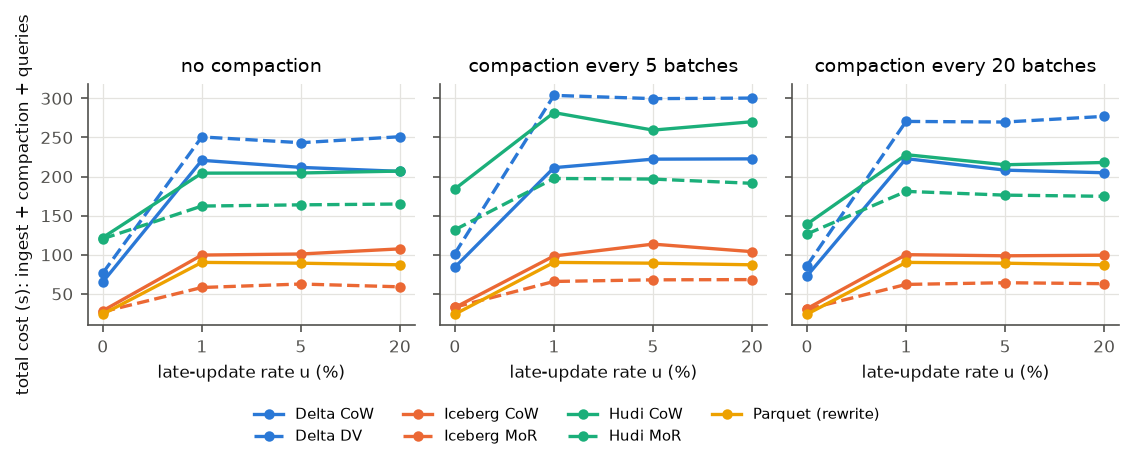
\includegraphics[width=\columnwidth]{fig_rq1_total_cost.png}
\caption{Total cost (ingest + compaction + all checkpoint queries; median of 5 runs, normalised to the reference
VM) versus late-update rate. Solid: copy-on-write; dashed: merge-on-read / deletion vectors.}
\label{fig:rq1}
\end{figure}
\textbf{The step is at $u>0$, not in $u$.} Moving from append-only ingestion to any late data multiplies total cost by
3.3--3.8$\times$ for the copy-on-write layouts (Delta 3.3, Iceberg 3.6, Parquet 3.8), by 3.3$\times$ for Delta DV,
2.2$\times$ for Iceberg MoR and 1.3--1.7$\times$ for Hudi (Fig.~\ref{fig:rq1}). Between $u=1\%$ and $u=20\%$ the cost
of every layout without compaction varies by at most 8\%. With $u=1\%$ a batch already carries 216 corrections scattered over the last 72
hours, i.e.\ over four day partitions holding only a few files each, so practically every file of those partitions
is touched. Copy-on-write then rewrites the same files whether 216 or 4{,}320 rows change; merge-on-read writes delete
markers whose number, not the rewritten volume, grows with $u$.

\textbf{Iceberg MoR is cheapest whenever $u>0$}: 59--63\,s, against 1.5$\times$ for plain Parquet,
1.6--1.8$\times$ for Iceberg CoW, 2.7--2.8$\times$ for Hudi MoR and 3.3--4.4$\times$ for the Delta and Hudi CoW
configurations. At $u=0$ the plain-Parquet baseline is fastest (24\,s), followed by both Iceberg modes (27--28\,s);
Hudi is slowest (122--123\,s) because its insert path merges new records into existing small files.
Ingest dominates total cost in our workload (40 batches against four checkpoints), so a layout's write path largely
decides RQ1; Section~\ref{sec:disc} discusses the break-even when queries are more frequent.

\begin{figure}[t]\centering
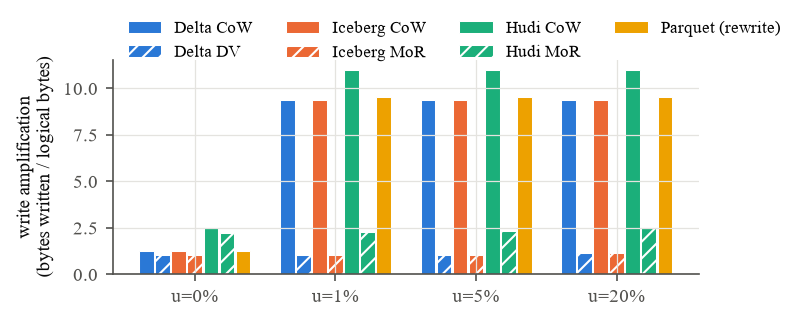
\includegraphics[width=\columnwidth]{fig_write_amplification.png}
\caption{Write amplification without compaction.}
\label{fig:wa}
\end{figure}
Write amplification (Fig.~\ref{fig:wa}) makes the mechanism visible. All copy-on-write layouts write about 9.4 times
the final table size once $u>0$ (Hudi CoW 11.0), independent of $u$; Delta DV and Iceberg MoR stay at 1.03--1.16,
growing slowly with $u$. Hudi MoR sits in between (2.3--2.5) even at $u=0$, because Hudi's small-file handling routes
new records into existing small base files and rewrites them. Bytes are not time, however: Delta DV writes 8$\times$
fewer bytes than Delta CoW yet ingests 10--13\% more slowly, whereas Iceberg MoR converts the same byte saving into a
nearly 2$\times$ faster ingest than Iceberg CoW. On local disk, the per-commit work of each format's MERGE implementation
matters more than the bytes it writes.

\subsection{Where the time goes}
Fig.~\ref{fig:breakdown} splits total cost at $u=20\%$ into ingest, compaction and checkpoint queries. Ingest accounts for 87--98\%
of the total without compaction, which explains why RQ1 is decided on the write path: Iceberg MoR is the only layout where queries
reach 13\% of the total, and even there they do not change its rank. With compaction every 20 batches the compaction bar is short
for Iceberg MoR (8\,s) and larger for Hudi and Delta DV (17--20\,s). The only change of rank is that Delta CoW passes Hudi CoW, whose clustering adds 18\,s; these two are statistically tied anyway.
Every run in this matrix issues four query rounds; Section~\ref{sec:disc} asks how the ranking changes with more reads.

\begin{figure*}[!t]\centering
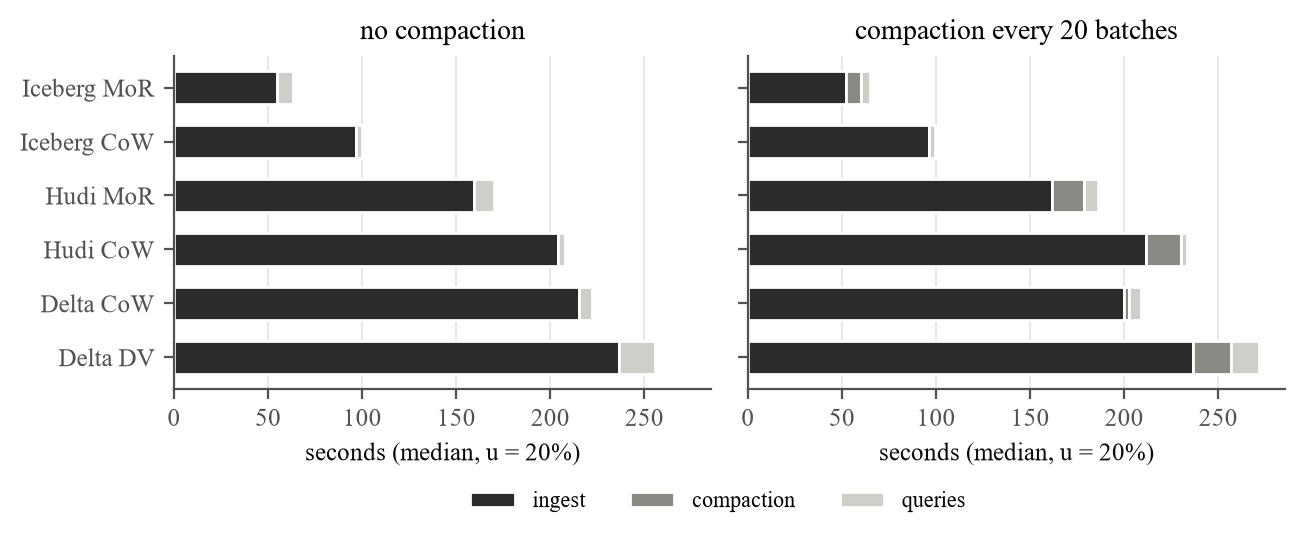
\includegraphics[width=0.8\textwidth]{fig_breakdown.png}
\caption{Breakdown of total cost at $u=20\%$ (medians of 5 runs, normalised). Components are medians taken separately, so bars may
differ from Table~\ref{tab:u20} totals by a second or two.}\label{fig:breakdown}
\end{figure*}

\subsection{RQ2: compaction cadence}
\begin{figure}[t]\centering
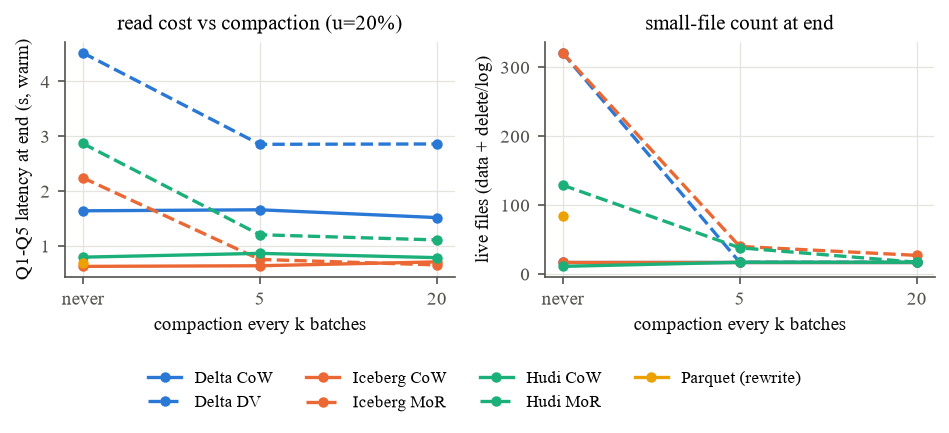
\includegraphics[width=\columnwidth]{fig_rq2_compaction.png}
\caption{Read latency at the end of the run and live file count versus compaction cadence ($u=20\%$).}
\label{fig:rq2}
\end{figure}
\begin{figure}[t]\centering
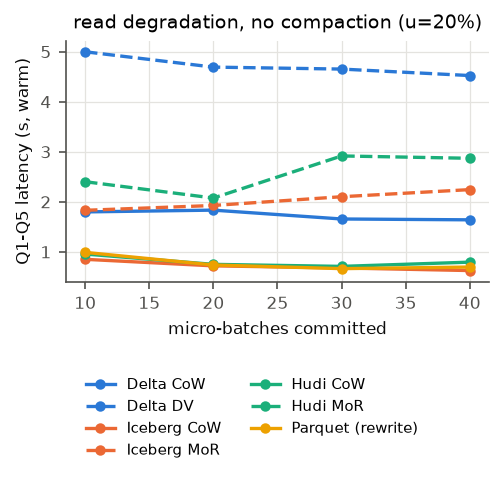
\includegraphics[width=0.75\columnwidth]{fig_rq2_degradation.png}
\caption{Warm Q1--Q5 latency over the run without compaction ($u=20\%$).}
\label{fig:deg}
\end{figure}
\textbf{Without compaction, merge-on-read pays at read time.} After 40 batches at $u=20\%$, Delta DV and Iceberg MoR
hold 167 data files plus 154 deletion vectors or delete files, and Hudi MoR 5 base files plus 124 log files, against
11--17 files for copy-on-write (Fig.~\ref{fig:rq2}, right). Warm Q1--Q5 latency is correspondingly 2.27\,s for Iceberg
MoR, 2.86\,s for Hudi MoR and 4.76\,s for Delta DV, versus 0.63, 0.80 and 1.64\,s for the copy-on-write mode of the
same format. Over the run (Fig.~\ref{fig:deg}) copy-on-write latency falls slightly as the JVM warms up
(degradation rate $-9$\% to $-26$\%), whereas Iceberg MoR rises by 28\% and Hudi MoR by 15\%; Hudi MoR jumps between
the 20th and 30th batch, which is where a break point in small-file count shows up in our data (H3).

\textbf{Compaction every 20 batches is the cheap option, not a free one.} Right after a compaction it brings Iceberg MoR
to 0.67\,s and Hudi MoR to 1.19\,s, i.e.\ 6\% and 49\% above their copy-on-write reads, for 8\,s (Iceberg) and 17\,s
(Hudi) of compaction over the run. These end-of-run figures flatter the cadence, however, because each checkpoint runs after
that batch's compaction. Fig.~\ref{fig:sawtooth} shows the checkpoint in between: ten batches after a compaction, reads are
back at 1.29\,s for Iceberg MoR and 2.13\,s for Hudi MoR, about 2.0$\times$ and 2.7$\times$ copy-on-write, so latency follows a
sawtooth. Averaged over the four checkpoints at $u=20\%$, Q1--Q5 take 2.06\,s without compaction, 1.13\,s with compaction every
20 batches and 0.84\,s every 5 batches on Iceberg MoR, against 0.72\,s for Iceberg CoW; on Hudi the figures are 2.58, 1.79, 1.21
and 0.84\,s. Compacting every 5 batches costs about twice as much (15 and 37\,s) and its total cost is not distinguishable from
every 20 batches at this query rate (Section~\ref{sec:stats}), but it keeps reads steadier. All its checkpoints also fall right after a compaction, so
its figures are a best case. We did not measure the very end of a 20-batch cycle, where latency should be higher than at the
midpoint. For copy-on-write layouts compaction buys nothing once $u>0$: every batch already
rewrites the touched partitions into one file each (17 files), and Iceberg's \texttt{rewrite\_data\_files} finds no
work. At $u=0$, by contrast, appends leave 47 files without compaction and compaction trims them to 17, with no
measurable change in read latency at this table size.

Two maintenance details matter in practice. First, Iceberg 1.6's \texttt{rewrite\_data\_files} rewrote the data but left
delete files that no longer apply: 23 (every 5 batches) and 10 (every 20 batches) remained live at the end, whereas Delta's
\texttt{REORG}+\texttt{OPTIMIZE} left none at either cadence; Hudi left none when compacting every 20 batches but 25
log files when compacting every 5. Second, enabling deletion vectors slows every Delta query by roughly 0.2--0.3\,s even
after all vectors have been purged (Q1--Q5: 2.86\,s versus 1.58\,s with the same 17 files), so a Delta table that is mostly read is better served by copy-on-write.

\begin{figure*}[!t]\centering
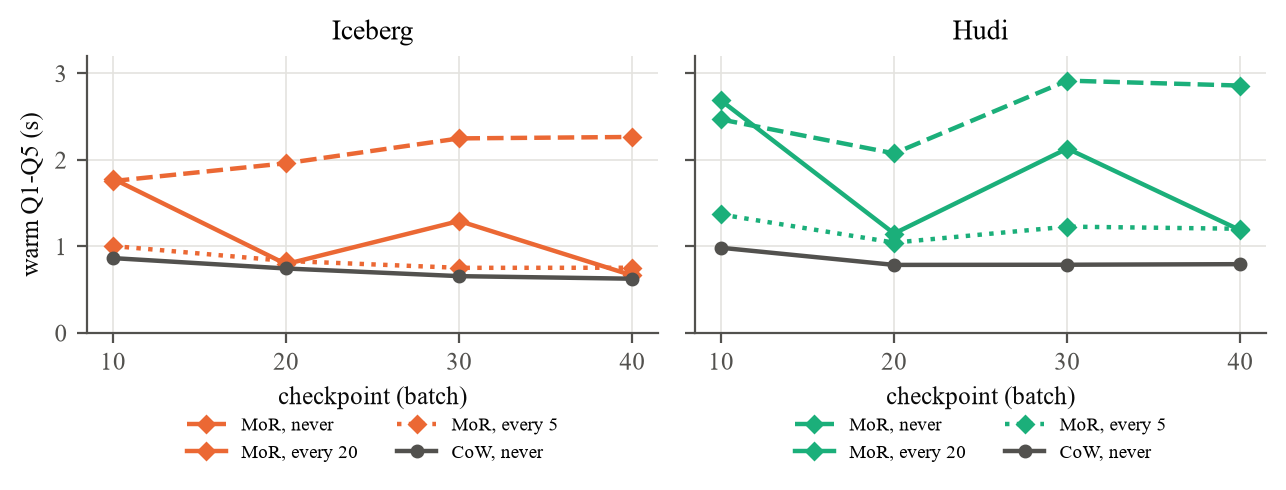
\includegraphics[width=0.8\textwidth]{fig_sawtooth.png}
\caption{Warm Q1--Q5 latency at each checkpoint, $u=20\%$. Every-20 readings at batches 20 and 40, and all every-5 readings, are taken
right after a compaction; the every-20 reading at batch 30 is ten batches after one.}\label{fig:sawtooth}
\end{figure*}

\subsection{RQ3: metadata and time travel}
\begin{figure}[t]\centering
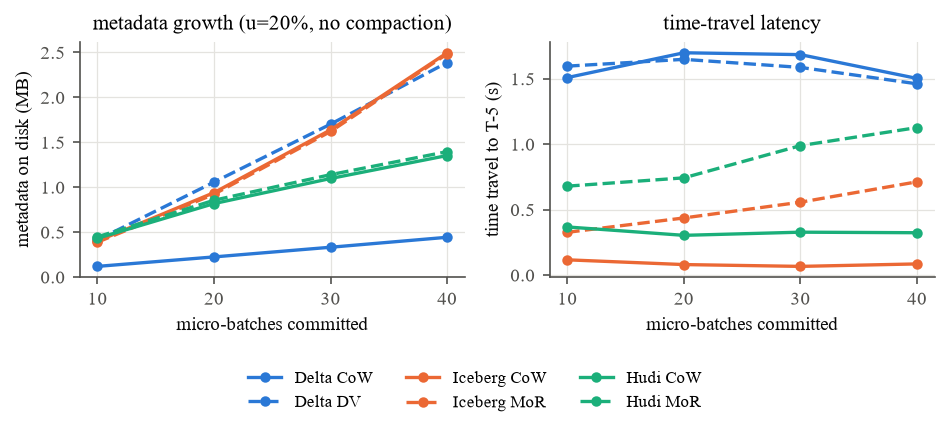
\includegraphics[width=\columnwidth]{fig_rq3_metadata.png}
\caption{Metadata on disk and time-travel latency (to the version 5 commits back) over the run ($u=20\%$, no
compaction; one batch adds about one commit, deletes and compactions add more).}
\label{fig:rq3}
\end{figure}
\textbf{Metadata grows linearly, at very different rates} (Fig.~\ref{fig:rq3}, left). Per micro-batch, Delta CoW's log
grows by 11\,KB (0.45\,MB after 45 versions), Hudi by 31--32\,KB (1.4\,MB), Delta DV by 67\,KB and Iceberg by 72\,KB in
either mode (2.4--2.5\,MB). Iceberg writes a new metadata JSON, manifest list and manifests per snapshot; Delta DV's log
grows six times faster than Delta CoW's because each commit re-adds every touched file with its new deletion vector, and
the DV table keeps ten times more live files (167 versus 17). Hudi's metadata keeps growing after its active timeline is
full, but only 23 versions remain reachable by time travel: older instants are archived even with the cleaner off.

\textbf{Time-travel latency follows the delete files, not the metadata size} (Fig.~\ref{fig:rq3}, right). Reading the
version five commits back takes 0.06--0.13\,s on Iceberg CoW and about 0.3\,s on Hudi CoW, flat over the run, and about
1.6\,s on Delta in both modes, also flat because Delta checkpoints its log every 10 commits. The two merge-on-read
formats that accumulate delete artefacts slow down as the run proceeds: Iceberg MoR from 0.33 to 0.71\,s and Hudi MoR
from 0.68 to 1.13\,s. Within 45 versions and 2.5\,MB, metadata size itself had no visible effect on latency.

\subsection{Cost of individual operations}
\begin{figure}[t]\centering
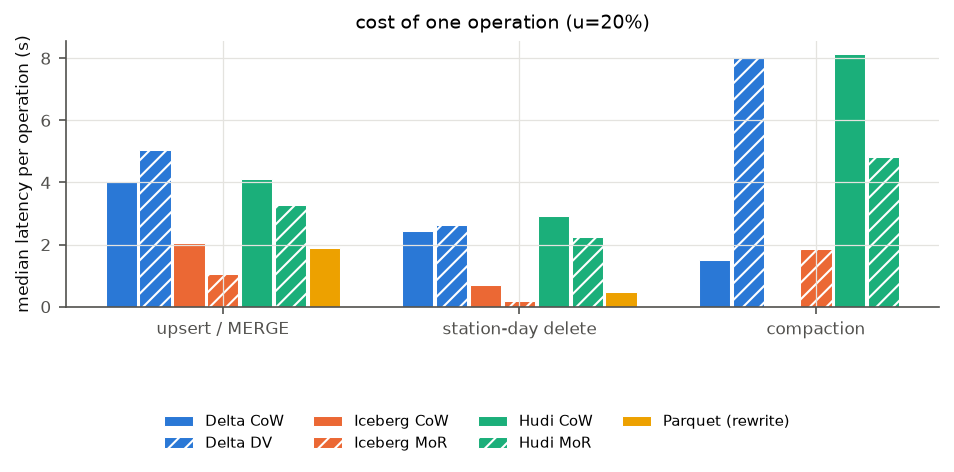
\includegraphics[width=\columnwidth]{fig_ops.png}
\caption{Median latency of one operation at $u=20\%$: a micro-batch upsert and a station-day delete (no compaction), and
one compaction (both cadences).}
\label{fig:ops}
\end{figure}
Fig.~\ref{fig:ops} breaks total cost down to single operations. A micro-batch MERGE with 4{,}320 corrections takes
1.05\,s on Iceberg MoR, 2.00\,s on Iceberg CoW, 1.89\,s on plain Parquet, 3.3--4.2\,s on Hudi and 4.5--5.0\,s on Delta.
Deleting one station-day is cheapest on Iceberg MoR (0.19\,s, a single position-delete file) and costs 2.2--2.9\,s on
Delta and Hudi in either mode: on Delta, the deletion vector saves the file rewrite but not the commit overhead, and on
Hudi the delete is itself an upsert of tombstones that must first be read from the table. One compaction costs 1.8\,s
on Iceberg MoR, 4.9\,s on Hudi MoR and about 8\,s on Delta DV (\texttt{REORG} plus \texttt{OPTIMIZE}) and Hudi CoW
(clustering); Iceberg CoW's compaction finds nothing to rewrite (0.03\,s). The initial bulk load of 604{,}800 rows takes
5.5--6.3\,s for Parquet and Iceberg, 10.3--10.4\,s for Delta and 12.9--13.0\,s for Hudi, consistent with LHBench's observation
that Hudi loads more slowly~\cite{jain2023lhbench}. JVM and session start-up, excluded from all totals, takes
2.7--3.8\,s per run.

\subsection{Ingest over time}
\begin{figure}[t]\centering
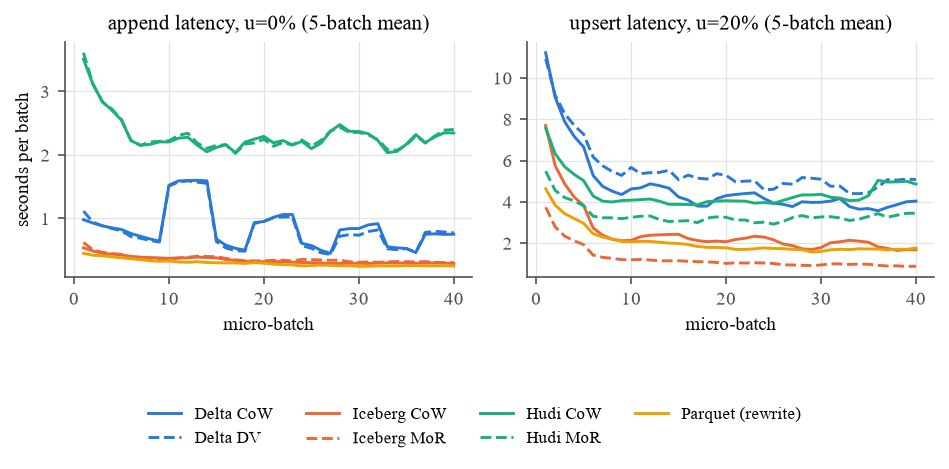
\includegraphics[width=\columnwidth]{fig_ingest_trend.png}
\caption{Per-batch ingest latency over the run without compaction (median of 5 runs, 5-batch moving mean).}
\label{fig:trend}
\end{figure}
Ingest latency does not grow as the table grows from 0.6 to 1.43\,M rows (Fig.~\ref{fig:trend}). The first batches are
slow while the JVM warms up; afterwards upsert latency is flat or slightly falling, e.g.\ Iceberg MoR 1.97\,s in
batches 1--5 and 0.90\,s in batches 36--40, Delta CoW 6.53 and 4.49\,s. The explicit \texttt{day IN (\dots)}
predicate confines every MERGE to the four newest day partitions, so its cost depends on the size of those partitions,
not of the table. Two patterns stand out. Delta's append latency jumps every tenth commit (5.1\,s at commit 10 and
2.7\,s at commit 20, versus 0.5\,s otherwise): the commit that writes the Parquet log checkpoint pays for it
synchronously. Hudi's append latency stays at 2.2--2.4\,s throughout, 7$\times$ Iceberg's, because small-file
handling merges each batch into existing base files.

\subsection{Which queries pay the merge-on-read penalty}
\begin{table}[t]\centering
\caption{Warm latency per query at the end of the run, $u=20\%$ (seconds, median of 5; the ``every 20'' rows are read right after a compaction)}\label{tab:perquery}
\footnotesize
\begin{tabular}{@{}lrrrrr@{}}\toprule
Layout (compaction) & Q1 & Q2 & Q3 & Q4 & Q5\\\midrule
Iceberg CoW (never) & 0.10 & 0.11 & 0.28 & 0.05 & 0.10\\
Iceberg MoR (never) & 0.14 & 0.24 & 1.15 & 0.08 & 0.74\\
Iceberg MoR (every 20) & 0.12 & 0.11 & 0.27 & 0.07 & 0.09\\
Hudi CoW (never) & 0.15 & 0.12 & 0.33 & 0.06 & 0.10\\
Hudi MoR (never) & 0.14 & 0.28 & 1.28 & 0.16 & 0.95\\
Hudi MoR (every 20) & 0.14 & 0.19 & 0.50 & 0.08 & 0.22\\
Delta CoW (never) & 0.28 & 0.29 & 0.54 & 0.25 & 0.33\\
Delta DV (never) & 0.84 & 0.81 & 1.46 & 0.68 & 0.85\\
Delta DV (every 20) & 0.54 & 0.46 & 0.81 & 0.53 & 0.49\\
Parquet (rewrite) & 0.12 & 0.12 & 0.28 & 0.06 & 0.10\\\bottomrule
\end{tabular}
\end{table}
Table~\ref{tab:perquery} shows where merge-on-read reads lose time. For Iceberg and Hudi the penalty is concentrated in
the queries that scan the whole history: Q3 (join over all days) is 3.9--4.1$\times$ slower than with copy-on-write and
Q5 (full scan) 7.7--9.5$\times$, because they open every data file together with its delete or log files. The
dashboard-style queries over recent data (Q1, Q4) are almost unaffected, since partition pruning limits them to one or
two days. Delta DV is different: all five queries are 2.6--3.0$\times$ slower than Delta CoW, which points to a per-query
cost of the deletion-vector read path rather than to the volume of deleted rows. Compaction every 20 batches removes
the Iceberg penalty completely and most of the Hudi penalty.

\subsection{Cold and warm queries}
Each query ran twice per checkpoint. At the end of the run, the first (cold) execution of Q1--Q5 took
1.2--2.1$\times$ as long as the second: 2.09$\times$ for Delta CoW, 1.69$\times$ for Hudi CoW, 1.49$\times$ for
Iceberg CoW, but only 1.18--1.42$\times$ for the merge-on-read layouts, whose cost is dominated by work that caching does
not remove (reading and applying delete or log files), and 1.24$\times$ for plain Parquet, which has no table metadata
to load. The cold-to-warm gap thus mainly reflects query planning and metadata loading.

\subsection{Append-only ingestion (\texorpdfstring{$u=0$}{u=0})}
Without late data, the two modes of each format differ little, because merge-on-read only matters for the four
deletes. Appends leave 47 files after 40 batches; compaction every 20 batches trims them to 17 at a total
cost of 3--9\,s for Iceberg and Delta, with no measurable change in read latency at this table size. Plain Parquet is
fastest (24\,s in total), Iceberg 27--28\,s, Delta 65--78\,s and Hudi 122--123\,s. For append-only monitoring feeds,
the choice of format is therefore driven by the features needed (atomicity, history, multi-engine access) rather than
by performance, except that Hudi's upsert-oriented write path costs 4--5$\times$ more than necessary.

%=====================================================================================================
\subsection{Ablation: removing one mechanism at a time}\label{sec:ablation}
Table~\ref{tab:ablation} switches off one mechanism while everything else stays the same. Read latency is the mean of the four
checkpoints, so it does not depend on the timing issue above. Removing compaction lowers total cost by 1--18\,s and raises mean
read latency by 0.8--1.0\,s: at four query rounds per run this is a net saving, which is why the cheapest total in our matrix is
the uncompacted table even though we recommend compaction. Removing deletion vectors from Delta is a clear gain on both axes: total
cost and reads both improve, so the mechanism has no benefit here. Removing Iceberg's position deletes has the opposite effect:
total cost rises by 37\,s while mean read latency falls by 1.3\,s, a genuine trade-off. Hudi's log files behave the same way.

A third ablation removes the normalisation by VM. Computed on raw seconds, the step from $u=0$ to $u=1\%$ reads 2.1--5.8$\times$
rather than 1.3--3.8$\times$, and cost appears to vary by 36--50\% between $u=1\%$ and $u=20\%$ rather than by at most 8\%. Without
calibration the central finding of RQ1, that the rate of late data hardly matters, would have been hidden by VM speed.

\begin{table}[!t]\centering
\caption{Ablation at $u=20\%$: total cost (s) and mean read latency over the four checkpoints (s), with the mechanism on and off}\label{tab:ablation}
\footnotesize\setlength{\tabcolsep}{3pt}
\begin{tabular}{@{}llrrrr@{}}\toprule
Removed & Layout & Total on & off & Read on & off\\\midrule
Compaction & Iceberg MoR & 64 & 63 & 1.13 & 2.06\\
Compaction & Hudi MoR & 186 & 170 & 1.79 & 2.58\\
Compaction & Delta DV & 273 & 256 & 3.87 & 4.85\\
Deletion vectors & Delta & 256 & 223 & 4.85 & 1.77\\
Position deletes & Iceberg & 63 & 100 & 2.06 & 0.72\\
Log files & Hudi & 170 & 208 & 2.58 & 0.84\\\bottomrule
\end{tabular}
\end{table}

\subsection{Statistical confidence}\label{sec:stats}
Table~\ref{tab:stats} tests the main claims. For each pair we report the ratio of medians, a 95\% bootstrap interval (20,000 resamples
of the five repetitions on each side) and an exact two-sided Mann--Whitney test. With five values per side that test cannot go below
$p=0.008$, which requires complete separation of the two groups. Every claim that Iceberg MoR beats another layout reaches this
limit at all three update rates, as does the claim that Delta DV ingests more slowly than Delta CoW. The flatness of cost between
$u=1\%$ and $u=20\%$ also survives: no layout shows a significant difference ($p\ge 0.095$; the two extremes are in the table).

Two results are weaker than they look in the medians. Delta CoW and Hudi CoW at $u=20\%$ differ by 7\% in the median, but the
interval spans 1 and $p=0.84$, so they are tied. The total-cost gap between compacting every 5 and every 20 batches is also not
significant ($p=0.15$), so the cheaper total of every 20 batches is a tendency rather than a firm result. We ran 26 such tests and
do not correct for multiple comparisons; with $n=5$ a Bonferroni correction would make none significant, so the table should be read as
effect sizes with honest uncertainty. The bootstrap on five values is coarse, and its intervals are not symmetric.

Fig.~\ref{fig:agreement} checks reproducibility across VMs. Each point compares one configuration's median over repetitions 1--3 with
its median over repetitions 4--5, which ran on different VMs six days later. All 76 configurations fall within $\pm$15\% of the diagonal
(0.89--1.12$\times$), and the median offset is 2\%.

\begin{table}[!t]\centering
\caption{Ratio of medians, 95\% bootstrap interval and exact Mann--Whitney $p$ ($n=5$ per side); $p=0.008$ is the lowest attainable}\label{tab:stats}
\footnotesize\setlength{\tabcolsep}{3pt}
\begin{tabular}{@{}lrcr@{}}\toprule
Comparison & Ratio & 95\% interval & $p$\\\midrule
Parquet / Ice.\ MoR, $u=1\%$ & 1.54 & [1.52, 1.81] & 0.008\\
Parquet / Ice.\ MoR, $u=20\%$ & 1.45 & [1.32, 1.57] & 0.008\\
Ice.\ CoW / Ice.\ MoR, $u=20\%$ & 1.58 & [1.46, 1.94] & 0.008\\
Hudi MoR / Ice.\ MoR, $u=20\%$ & 2.69 & [2.51, 2.97] & 0.008\\
Delta DV / CoW, ingest, $u=20\%$ & 1.10 & [1.04, 1.26] & 0.008\\
Delta CoW / Hudi CoW, $u=20\%$ & 1.07 & [0.91, 1.11] & 0.841\\
Ice.\ MoR, $u=20\%$ / $1\%$ & 1.08 & [1.00, 1.13] & 0.095\\
Delta CoW, $u=20\%$ / $1\%$ & 1.03 & [0.89, 1.10] & 0.841\\
Ice.\ MoR, total, every 5 / 20 & 1.05 & [0.97, 1.13] & 0.151\\
Hudi MoR, total, every 5 / 20 & 1.03 & [0.95, 1.16] & 0.151\\
Ice.\ MoR, end read, never / 20 & 3.41 & [3.04, 3.80] & 0.008\\
Hudi MoR, end read, never / 20 & 2.41 & [1.41, 3.22] & 0.008\\\bottomrule
\end{tabular}
\end{table}

\begin{figure}[!t]\centering
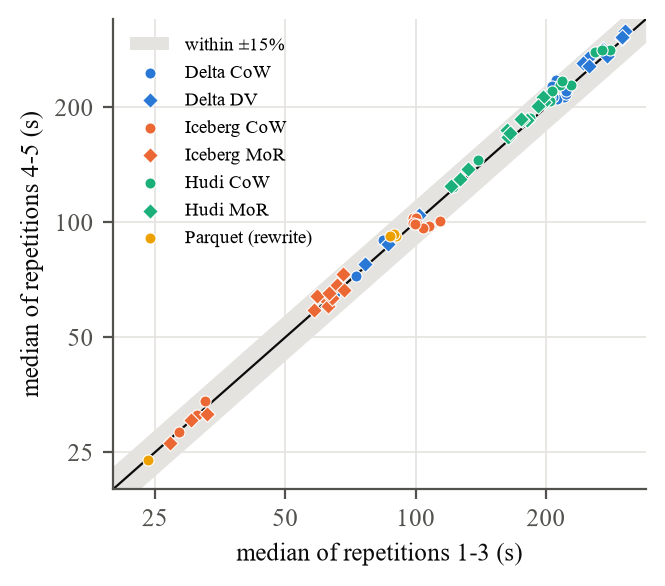
\includegraphics[width=0.85\columnwidth]{fig_rep_agreement.png}
\caption{Agreement between the two VM batches after normalisation: one point per configuration, shaded band $\pm$15\%.}\label{fig:agreement}
\end{figure}

\section{Discussion}\label{sec:disc}
\subsection{Explaining the differences}
\emph{Iceberg MoR} turns a MERGE into new data files for the changed rows plus small position-delete files, and plans
queries from manifests without a separate log replay; its write path is the lightest of all layouts, and its read
penalty is removed by a cheap \texttt{rewrite\_data\_files}. \emph{Delta Lake} pays a fixed per-commit and per-query
cost: its MERGE first joins to find the touched files and then rewrites or marks them, and every snapshot is
reconstructed from the log. Deletion vectors remove the rewrite volume but not this fixed cost, and add their own
overhead on reads, which is why they did not pay off at gigabyte scale on local disk; on object storage, where
bytes cost more, the balance may differ. \emph{Hudi} routes every record through its key index, and its small-file
handling merges new records into existing base files; this gives the highest write amplification in CoW mode
(11.0) and makes even append-only ingestion the slowest, while its MoR mode recovers part of the cost by deferring
merges to log files. \emph{Plain Parquet} has no metadata cost and rewrites whole partitions, which beats Delta and
Hudi here but offers no atomicity: a reader during a partition swap sees missing data, and no history is kept.

\textbf{Query frequency.} Our checkpoints run Q1--Q5 four times per 40 batches. A dashboard that refreshes more often
weights reads more heavily. Table~\ref{tab:breakeven} turns the measurements into a break-even point: the number of Q1--Q5 rounds
per 40 batches at which the write-side saving of a merge-on-read layout over copy-on-write equals its read penalty, taking the mean
latency of the four checkpoints as the cost of one round. Iceberg MoR without compaction stops paying off at 32--41 rounds, about
one per batch; with compaction every 20 batches it holds up to 83--111 rounds. Hudi MoR breaks even at 26--53 rounds in both cases.
Between the two Iceberg cadences, the extra 7--8\,s of compaction every 5 batches saves 0.28--0.36\,s per round and repays itself
after 21--28 rounds per 40 batches. The practical rule is therefore a simple one: compact every 20 batches when dashboards refresh
less often than every second batch, and every 5 batches when they refresh more often. This model is deliberately simple. It
treats reads as independent of ingest, ignores concurrency, and inherits the checkpoint timing discussed above, which favours the
every-5 cadence.

\begin{table}[!t]\centering
\caption{Break-even of merge-on-read against copy-on-write of the same format, $u=1$--$20\%$: write-side saving (s per run), mean read penalty
(s per Q1--Q5 round) and Q1--Q5 rounds per 40 batches at which they cancel out}\label{tab:breakeven}
\footnotesize\setlength{\tabcolsep}{3pt}
\begin{tabular}{@{}llrrr@{}}\toprule
Layout & Compaction & Saving & Penalty & Rounds\\\midrule
Iceberg MoR & never & 42--49 & 1.20--1.40 & 32--41\\
Iceberg MoR & every 20 & 37--42 & 0.38--0.46 & 83--111\\
Iceberg MoR & every 5 & 33--36 & 0.09--0.11 & 292--395\\
Hudi MoR & never & 45--49 & 0.92--1.74 & 26--53\\
Hudi MoR & every 20 & 24--29 & 0.57--0.95 & 27--50\\
Hudi MoR & every 5 & 1--16 & 0.34--0.37 & 2--43\\\bottomrule
\end{tabular}
\end{table}

\subsection{Relation to LHBench and LST-Bench}
LHBench found that on TPC-DS at 3\,TB the formats differ mainly in data read time~\cite{jain2023lhbench}. Our
workload reverses the emphasis: with 222\,MB of data, scans are short, and what separates the layouts is the write
path---how much is rewritten per correction and how much fixed work each commit costs. This does not contradict
LHBench; it shows that the conclusion depends on the ratio of writes to reads and on table size, which is why
update-heavy, small-scale deployments need their own measurements. We confirm LHBench's observation that Hudi loads
more slowly, and extend it: at small scale Hudi is also the slowest for plain appends, because of small-file handling.
In the spirit of LST-Bench's stability metrics~\cite{camacho2024lstbench}, we found no long-term degradation of
ingest, while read degradation of merge-on-read tables is real but bounded by modest compaction.

\subsection{Practical pitfalls}
Several behaviours that are easy to miss changed either results or correctness in our runs:
\begin{enumerate}
\item \emph{Hudi timestamp keys.} With a timestamp in a composite record key, Hudi's bulk-insert path and its upsert
path rendered the key differently (one used the JVM's local time zone), so upserts inserted duplicates instead of
updating. Only the checksum revealed it; we key on a string \texttt{id\_station|epoch\_micros}.
\item \emph{Hudi compaction trigger.} By default Hudi schedules compaction only after five delta commits, so an
explicit compaction call may silently do nothing; the cadence must be set explicitly.
\item \emph{Hudi archiving.} Even with the cleaner disabled, archiving keeps only about 23 instants reachable. With a
commit every few minutes, as in a real monitoring feed, that is a time-travel horizon of one to two hours unless the
archiving window is raised.
\item \emph{Iceberg dangling deletes.} \texttt{rewrite\_data\_files} in Iceberg 1.6 leaves position-delete files that
no longer apply; they count against planning and storage until removed.
\item \emph{Delta log checkpoints.} Every tenth commit writes the log checkpoint synchronously and is several times
slower than other commits, a latency spike that matters for ingestion with deadlines.
\item \emph{Different defaults.} Iceberg writes zstd and Hudi gzip by default, Spark and Delta snappy; comparisons
that keep defaults partly measure compression codecs.
\end{enumerate}

\subsection{Towards object storage and clusters}
Our runs use local disk on one node. On object storage each file costs a request and listing is slow, so the number
of files and metadata objects weighs more, and bytes written cost bandwidth. We expect this to (i)~widen the gap
between copy-on-write (9--11$\times$ the bytes) and merge-on-read, (ii)~penalise merge-on-read tables without
compaction more strongly, because every delete or log file is another request, and (iii)~make Iceberg's per-snapshot
metadata files and Hudi's metadata table more visible. Deletion vectors, which saved bytes but not time here, may pay
off on object storage. These are hypotheses for the multi-node MinIO setup planned as future work.

\subsection{Decision table}
\begin{table}[ht]\centering
\caption{Recommended configuration for a small monitoring deployment (single node, $\le$ a few GB per day)}\label{tab:decision}
\footnotesize
\begin{tabular}{@{}p{2.6cm}p{2.7cm}p{2.2cm}@{}}\toprule
Situation & Layout & Compaction\\\midrule
Append-only ($u=0$), ACID/history needed & Iceberg (either mode) & every 20 batches\\
Append-only, no ACID needed & plain Parquet & --\\
Any late data ($u=1$--$20\%$) & Iceberg MoR & every 20 batches; every 5 if read-heavy\\
Already on Delta Lake & Delta CoW (DV off) & optional\\
Already on Hudi & Hudi MoR & every 20 batches\\
Long time-travel horizon & Iceberg or Delta (Hudi keeps $\approx$23 versions by default) & --\\\bottomrule
\end{tabular}
\end{table}

\subsection{Threats to validity}
\emph{Scale and hardware.} One 4-vCPU VM and local disk, not a multi-node cluster on object storage; network and
object-store latency (which penalise many small files and metadata round trips) are absent, so our small-file
penalties are a lower bound. \emph{Shared VMs.} Cloud notebooks are shared machines; repeated identical queries can
vary widely in runtime on cloud hardware, so we use repetitions, randomised interleaving and a calibration
configuration, and report CV. Normalising by one calibration factor per VM assumes all layouts slow down alike on
a slower VM; comparisons between layouts never rely on it, because they are made within a VM. \emph{Versions and defaults.} Results hold for the pinned versions; we changed only
compression, cleaning and Hudi's compaction trigger, and report every setting. \emph{Data.} d1 values are
near-uniform and compress poorly; real sensor data would shrink absolute bytes. \emph{Engine.} Spark only; other
engines (Trino, DuckDB) may favour different formats. \emph{Scope against the proposal.} We repeat each configuration
five times as proposed, but repetitions 1--3 and 4--5 ran on different VMs, so the CV includes normalisation error; after normalisation the
median of repetitions 4--5 is about 2\% above that of repetitions 1--3 ($\pm$12\% per configuration). With five samples p95 is close to the
maximum and remains indicative only (total cost at $u=20\%$ without compaction: 66\,s for Iceberg MoR, 178\,s for Hudi MoR, 266\,s for Delta DV). A batch holds 6 hours of data instead of 1--5 minutes,
so results reflect the cost per batch size, not a minutes-level write cadence. We did not vary target file size,
partitioning by station and day, or Z-ordering, and did not run a default-configuration baseline; each day partition
is about 13\,MB, so every file is below 128\,MB. \sys{} runs standalone and is not yet integrated into LST-Bench.

%=====================================================================================================
\section{Conclusion and Future Work}\label{sec:concl}
For update-heavy sensor tables on a single node, the presence of late data, not its rate, sets the cost: total cost
jumps 1.3--3.8$\times$ when corrections appear and then stays within 8\% from 1\% to 20\% late rows (RQ1). Iceberg
merge-on-read was the cheapest layout for every non-zero rate, and compacting it every 20 micro-batches returned reads to near
copy-on-write latency for 8--17\,s of work, although latency climbs again between compactions, so read-heavy dashboards should compact every 5 batches (RQ2).
Metadata grew linearly at 11--72\,KB per batch without affecting time-travel latency, which instead tracked the number
of delete or log files; Hudi's default archiving limits time travel to about 23 versions (RQ3). Delta's deletion
vectors reduced bytes written eightfold but not time, a reminder that byte-based metrics alone mislead on local disk.
Future work: multi-engine reads (Trino, DuckDB over Iceberg),
catalogs (Polaris, Unity Catalog), object storage (MinIO) on a 3--4 node cluster, and budget-aware compaction
policies in the style of AutoComp.

\section*{Reproducibility}
Code, staged-workload generator, notebooks, raw run JSONs and analysis scripts: \url{https://github.com/vinhha195-oss/lakehouse-p1}.

The full experiment needs no local cluster. Table~\ref{tab:repro} lists the steps; each Kaggle notebook is self-contained and embeds the
\texttt{sensorlst} package, so it can be re-run from a browser. The workload generator is deterministic for a given seed, so all layouts and
all repetitions read byte-identical input. The raw JSON record of every run is kept in the repository, and all tables and figures here, including
the statistics, are regenerated from these records by the two analysis commands.

\begin{table}[!t]\centering
\caption{Steps to reproduce the results}\label{tab:repro}
\scriptsize\setlength{\tabcolsep}{3pt}
\begin{tabular}{@{}p{1.9cm}p{6.3cm}@{}}\toprule
Step & Command or artefact\\\midrule
Run repetitions 1--3 & \texttt{notebooks/sensorlst\_u\{00,01,05,20\}.ipynb} on Kaggle CPU\\
Run repetitions 4--5 & \texttt{notebooks/sensorlst\_u\{00,01,05,20\}b.ipynb}\\
Aggregate & \texttt{python -m sensorlst.analyze results/kaggle/u*/runs\_u* --out results/report}\\
Extra analyses & \texttt{python scripts/extra\_analysis.py results/report}\\
Live demo & \texttt{run\_demo.bat}, then \texttt{http://localhost:8501}\\\bottomrule
\end{tabular}
\end{table}

\appendices
\section{Full Results}
Tables~\ref{tab:a-total}--\ref{tab:a-cv} give every configuration of the matrix. Read latencies are taken at the last checkpoint and therefore
right after a compaction for the ``5'' and ``20'' columns (Section~\ref{sec:results}). Plain Parquet has no compaction, so its other columns are empty.

\begin{table*}[!t]\centering
\caption{Total cost, s (median of 5, normalised). Columns: compaction every $k$ batches, $\infty$ = never}\label{tab:a-total}
\footnotesize
\begin{tabular}{@{}lrrrrrrrrrrrr@{}}\toprule
 & \multicolumn{3}{c}{$u=0$} & \multicolumn{3}{c}{$u=1\%$} & \multicolumn{3}{c}{$u=5\%$} & \multicolumn{3}{c}{$u=20\%$}\\
\cmidrule(lr){2-4}\cmidrule(lr){5-7}\cmidrule(lr){8-10}\cmidrule(lr){11-13}
Layout & $\infty$ & 5 & 20 & $\infty$ & 5 & 20 & $\infty$ & 5 & 20 & $\infty$ & 5 & 20\\\midrule
Iceberg MoR & 27 & 33 & 30 & 59 & 67 & 62 & 61 & 68 & 64 & 63 & 68 & 64\\
Iceberg CoW & 28 & 34 & 31 & 102 & 101 & 101 & 101 & 108 & 99 & 100 & 97 & 99\\
Hudi MoR & 122 & 135 & 129 & 163 & 205 & 182 & 164 & 207 & 184 & 170 & 193 & 186\\
Hudi CoW & 123 & 186 & 144 & 209 & 282 & 228 & 206 & 273 & 219 & 208 & 278 & 233\\
Delta CoW & 65 & 88 & 73 & 217 & 219 & 223 & 212 & 220 & 208 & 223 & 223 & 210\\
Delta DV & 78 & 102 & 87 & 256 & 308 & 272 & 248 & 300 & 277 & 256 & 302 & 273\\
Parquet & 24 & -- & -- & 90 & -- & -- & 93 & -- & -- & 92 & -- & --\\\bottomrule
\end{tabular}
\end{table*}

\begin{table*}[!t]\centering
\caption{Ingest time, s (median of 5, normalised)}\label{tab:a-write}
\footnotesize
\begin{tabular}{@{}lrrrrrrrrrrrr@{}}\toprule
 & \multicolumn{3}{c}{$u=0$} & \multicolumn{3}{c}{$u=1\%$} & \multicolumn{3}{c}{$u=5\%$} & \multicolumn{3}{c}{$u=20\%$}\\
\cmidrule(lr){2-4}\cmidrule(lr){5-7}\cmidrule(lr){8-10}\cmidrule(lr){11-13}
Layout & $\infty$ & 5 & 20 & $\infty$ & 5 & 20 & $\infty$ & 5 & 20 & $\infty$ & 5 & 20\\\midrule
Iceberg MoR & 22 & 22 & 22 & 51 & 48 & 50 & 52 & 49 & 52 & 55 & 49 & 52\\
Iceberg CoW & 24 & 24 & 24 & 99 & 98 & 98 & 98 & 104 & 95 & 97 & 94 & 96\\
Hudi MoR & 116 & 117 & 117 & 156 & 160 & 159 & 157 & 162 & 161 & 159 & 152 & 162\\
Hudi CoW & 119 & 118 & 121 & 205 & 210 & 205 & 203 & 205 & 199 & 204 & 210 & 212\\
Delta CoW & 57 & 55 & 57 & 210 & 198 & 213 & 205 & 201 & 199 & 215 & 202 & 200\\
Delta DV & 57 & 52 & 57 & 237 & 233 & 236 & 229 & 226 & 238 & 236 & 229 & 237\\
Parquet & 20 & -- & -- & 87 & -- & -- & 90 & -- & -- & 89 & -- & --\\\bottomrule
\end{tabular}
\end{table*}

\begin{table*}[!t]\centering
\caption{Compaction time over the whole run, s (median of 5, normalised)}\label{tab:a-compact}
\footnotesize
\begin{tabular}{@{}lrrrrrrrrrrrr@{}}\toprule
 & \multicolumn{3}{c}{$u=0$} & \multicolumn{3}{c}{$u=1\%$} & \multicolumn{3}{c}{$u=5\%$} & \multicolumn{3}{c}{$u=20\%$}\\
\cmidrule(lr){2-4}\cmidrule(lr){5-7}\cmidrule(lr){8-10}\cmidrule(lr){11-13}
Layout & $\infty$ & 5 & 20 & $\infty$ & 5 & 20 & $\infty$ & 5 & 20 & $\infty$ & 5 & 20\\\midrule
Iceberg MoR & 0.0 & 7.1 & 4.5 & 0.0 & 15.7 & 7.7 & 0.0 & 15.2 & 7.7 & 0.0 & 14.8 & 7.9\\
Iceberg CoW & 0.0 & 6.0 & 3.4 & 0.0 & 0.4 & 0.2 & 0.0 & 0.4 & 0.2 & 0.0 & 0.3 & 0.2\\
Hudi MoR & 0.0 & 12.2 & 5.7 & 0.0 & 39.4 & 17.2 & 0.0 & 40.1 & 16.7 & 0.0 & 36.6 & 17.0\\
Hudi CoW & 0.0 & 64.9 & 18.2 & 0.0 & 71.4 & 19.7 & 0.0 & 61.4 & 17.7 & 0.0 & 64.9 & 18.2\\
Delta CoW & 0.0 & 25.3 & 7.6 & 0.0 & 13.0 & 3.1 & 0.0 & 12.1 & 2.7 & 0.0 & 12.8 & 3.0\\
Delta DV & 0.0 & 37.6 & 13.4 & 0.0 & 64.9 & 20.7 & 0.0 & 64.1 & 19.0 & 0.0 & 65.1 & 19.9\\
Parquet & 0.0 & -- & -- & 0.0 & -- & -- & 0.0 & -- & -- & 0.0 & -- & --\\\bottomrule
\end{tabular}
\end{table*}

\begin{table*}[!t]\centering
\caption{Warm Q1--Q5 latency at the last checkpoint, s (median of 5, normalised)}\label{tab:a-read}
\footnotesize
\begin{tabular}{@{}lrrrrrrrrrrrr@{}}\toprule
 & \multicolumn{3}{c}{$u=0$} & \multicolumn{3}{c}{$u=1\%$} & \multicolumn{3}{c}{$u=5\%$} & \multicolumn{3}{c}{$u=20\%$}\\
\cmidrule(lr){2-4}\cmidrule(lr){5-7}\cmidrule(lr){8-10}\cmidrule(lr){11-13}
Layout & $\infty$ & 5 & 20 & $\infty$ & 5 & 20 & $\infty$ & 5 & 20 & $\infty$ & 5 & 20\\\midrule
Iceberg MoR & 1.09 & 0.82 & 0.79 & 2.15 & 0.77 & 0.74 & 2.47 & 0.74 & 0.71 & 2.27 & 0.75 & 0.67\\
Iceberg CoW & 0.97 & 0.82 & 0.77 & 0.66 & 0.69 & 0.70 & 0.66 & 0.69 & 0.71 & 0.63 & 0.64 & 0.71\\
Hudi MoR & 1.26 & 1.12 & 1.23 & 1.92 & 1.21 & 1.25 & 1.96 & 1.25 & 1.12 & 2.86 & 1.20 & 1.19\\
Hudi CoW & 0.78 & 0.77 & 0.83 & 0.83 & 0.85 & 0.88 & 0.81 & 0.77 & 0.79 & 0.80 & 0.86 & 0.79\\
Delta CoW & 2.08 & 1.71 & 1.75 & 1.72 & 1.65 & 1.52 & 1.60 & 1.62 & 1.58 & 1.64 & 1.66 & 1.58\\
Delta DV & 4.51 & 2.69 & 2.72 & 4.77 & 2.77 & 2.81 & 4.57 & 2.55 & 2.75 & 4.76 & 2.74 & 2.86\\
Parquet & 0.86 & -- & -- & 0.71 & -- & -- & 0.72 & -- & -- & 0.70 & -- & --\\\bottomrule
\end{tabular}
\end{table*}

\begin{table*}[!t]\centering
\caption{Write amplification (deterministic across repetitions)}\label{tab:a-wa}
\footnotesize
\begin{tabular}{@{}lrrrrrrrrrrrr@{}}\toprule
 & \multicolumn{3}{c}{$u=0$} & \multicolumn{3}{c}{$u=1\%$} & \multicolumn{3}{c}{$u=5\%$} & \multicolumn{3}{c}{$u=20\%$}\\
\cmidrule(lr){2-4}\cmidrule(lr){5-7}\cmidrule(lr){8-10}\cmidrule(lr){11-13}
Layout & $\infty$ & 5 & 20 & $\infty$ & 5 & 20 & $\infty$ & 5 & 20 & $\infty$ & 5 & 20\\\midrule
Iceberg MoR & 1.02 & 1.99 & 1.84 & 1.04 & 3.45 & 2.22 & 1.06 & 3.47 & 2.24 & 1.16 & 3.57 & 2.34\\
Iceberg CoW & 1.24 & 1.99 & 1.84 & 9.37 & 9.37 & 9.37 & 9.37 & 9.37 & 9.37 & 9.37 & 9.37 & 9.37\\
Hudi MoR & 2.24 & 2.44 & 2.44 & 2.29 & 4.22 & 3.24 & 2.34 & 4.26 & 3.29 & 2.51 & 4.44 & 3.46\\
Hudi CoW & 2.49 & 7.80 & 4.01 & 10.99 & 16.34 & 12.52 & 10.99 & 16.34 & 12.52 & 11.00 & 16.36 & 12.53\\
Delta CoW & 1.24 & 1.99 & 1.84 & 9.37 & 9.37 & 9.37 & 9.37 & 9.37 & 9.37 & 9.37 & 9.37 & 9.37\\
Delta DV & 1.02 & 1.99 & 1.84 & 1.03 & 5.55 & 3.14 & 1.06 & 5.57 & 3.17 & 1.16 & 5.65 & 3.27\\
Parquet & 1.24 & -- & -- & 9.54 & -- & -- & 9.53 & -- & -- & 9.53 & -- & --\\\bottomrule
\end{tabular}
\end{table*}

\begin{table*}[!t]\centering
\caption{Live delete, deletion-vector or log files at the end of the run}\label{tab:a-del}
\footnotesize
\begin{tabular}{@{}lrrrrrrrrrrrr@{}}\toprule
 & \multicolumn{3}{c}{$u=0$} & \multicolumn{3}{c}{$u=1\%$} & \multicolumn{3}{c}{$u=5\%$} & \multicolumn{3}{c}{$u=20\%$}\\
\cmidrule(lr){2-4}\cmidrule(lr){5-7}\cmidrule(lr){8-10}\cmidrule(lr){11-13}
Layout & $\infty$ & 5 & 20 & $\infty$ & 5 & 20 & $\infty$ & 5 & 20 & $\infty$ & 5 & 20\\\midrule
Iceberg MoR & 4 & 4 & 4 & 154 & 23 & 10 & 154 & 23 & 10 & 154 & 23 & 10\\
Iceberg CoW & 0 & 0 & 0 & 0 & 0 & 0 & 0 & 0 & 0 & 0 & 0 & 0\\
Hudi MoR & 4 & 1 & 0 & 124 & 25 & 0 & 124 & 25 & 0 & 124 & 25 & 0\\
Hudi CoW & 0 & 0 & 0 & 0 & 0 & 0 & 0 & 0 & 0 & 0 & 0 & 0\\
Delta CoW & 0 & 0 & 0 & 0 & 0 & 0 & 0 & 0 & 0 & 0 & 0 & 0\\
Delta DV & 4 & 0 & 0 & 73 & 0 & 0 & 142 & 0 & 0 & 154 & 0 & 0\\
Parquet & 0 & -- & -- & 0 & -- & -- & 0 & -- & -- & 0 & -- & --\\\bottomrule
\end{tabular}
\end{table*}

\begin{table*}[!t]\centering
\caption{Metadata on disk at the end of the run, KB}\label{tab:a-meta}
\footnotesize
\begin{tabular}{@{}lrrrrrrrrrrrr@{}}\toprule
 & \multicolumn{3}{c}{$u=0$} & \multicolumn{3}{c}{$u=1\%$} & \multicolumn{3}{c}{$u=5\%$} & \multicolumn{3}{c}{$u=20\%$}\\
\cmidrule(lr){2-4}\cmidrule(lr){5-7}\cmidrule(lr){8-10}\cmidrule(lr){11-13}
Layout & $\infty$ & 5 & 20 & $\infty$ & 5 & 20 & $\infty$ & 5 & 20 & $\infty$ & 5 & 20\\\midrule
Iceberg MoR & 2038 & 3057 & 2530 & 2545 & 4871 & 3646 & 2545 & 4868 & 3644 & 2543 & 4863 & 3639\\
Iceberg CoW & 2079 & 3059 & 2551 & 2556 & 2556 & 2556 & 2556 & 2556 & 2556 & 2556 & 2556 & 2556\\
Hudi MoR & 1207 & 1320 & 1267 & 1428 & 1574 & 1510 & 1429 & 1575 & 1511 & 1429 & 1575 & 1511\\
Hudi CoW & 1205 & 1362 & 1302 & 1384 & 1638 & 1481 & 1384 & 1639 & 1481 & 1385 & 1639 & 1481\\
Delta CoW & 225 & 279 & 243 & 453 & 453 & 453 & 453 & 453 & 453 & 453 & 453 & 453\\
Delta DV & 229 & 292 & 255 & 1402 & 1128 & 1345 & 2038 & 1355 & 1910 & 2445 & 1484 & 2277\\
Parquet & 0 & -- & -- & 0 & -- & -- & 0 & -- & -- & 0 & -- & --\\\bottomrule
\end{tabular}
\end{table*}

\begin{table*}[!t]\centering
\caption{Coefficient of variation of total cost over five repetitions}\label{tab:a-cv}
\footnotesize
\begin{tabular}{@{}lrrrrrrrrrrrr@{}}\toprule
 & \multicolumn{3}{c}{$u=0$} & \multicolumn{3}{c}{$u=1\%$} & \multicolumn{3}{c}{$u=5\%$} & \multicolumn{3}{c}{$u=20\%$}\\
\cmidrule(lr){2-4}\cmidrule(lr){5-7}\cmidrule(lr){8-10}\cmidrule(lr){11-13}
Layout & $\infty$ & 5 & 20 & $\infty$ & 5 & 20 & $\infty$ & 5 & 20 & $\infty$ & 5 & 20\\\midrule
Iceberg MoR & 0.031 & 0.028 & 0.019 & 0.009 & 0.030 & 0.017 & 0.023 & 0.069 & 0.011 & 0.053 & 0.048 & 0.038\\
Iceberg CoW & 0.018 & 0.025 & 0.024 & 0.030 & 0.038 & 0.027 & 0.035 & 0.064 & 0.027 & 0.109 & 0.067 & 0.048\\
Hudi MoR & 0.023 & 0.028 & 0.021 & 0.062 & 0.033 & 0.025 & 0.044 & 0.048 & 0.035 & 0.042 & 0.030 & 0.071\\
Hudi CoW & 0.034 & 0.014 & 0.033 & 0.028 & 0.015 & 0.003 & 0.046 & 0.047 & 0.033 & 0.047 & 0.047 & 0.059\\
Delta CoW & 0.009 & 0.052 & 0.087 & 0.046 & 0.093 & 0.067 & 0.038 & 0.087 & 0.046 & 0.069 & 0.049 & 0.044\\
Delta DV & 0.045 & 0.020 & 0.015 & 0.040 & 0.026 & 0.031 & 0.037 & 0.031 & 0.038 & 0.035 & 0.046 & 0.047\\
Parquet & 0.017 & -- & -- & 0.076 & -- & -- & 0.032 & -- & -- & 0.053 & -- & --\\\bottomrule
\end{tabular}
\end{table*}

\begin{thebibliography}{99}
\bibitem{oneil1996lsm} P.~O'Neil, E.~Cheng, D.~Gawlick, and E.~O'Neil, ``The log-structured merge-tree (LSM-tree),''
\emph{Acta Informatica}, vol.~33, no.~4, pp.~351--385, 1996.
\bibitem{jensen2017tsms} S.~K. Jensen, T.~B. Pedersen, and C.~Thomsen, ``Time series management systems: A survey,''
\emph{IEEE Trans. Knowl. Data Eng.}, vol.~29, no.~11, pp.~2581--2600, 2017.
\bibitem{leitner2016chaos} P.~Leitner and J.~Cito, ``Patterns in the chaos---a study of performance variation and
predictability in public IaaS clouds,'' \emph{ACM Trans. Internet Technol.}, vol.~16, no.~3, 2016.
\bibitem{uta2020reproducible} A.~Uta \emph{et al.}, ``Is big data performance reproducible in modern cloud
networks?'' in \emph{Proc. NSDI}, 2020.
\bibitem{armbrust2015sparksql} M.~Armbrust \emph{et al.}, ``Spark SQL: Relational data processing in Spark,'' in
\emph{Proc. SIGMOD}, 2015.
\bibitem{armbrust2021lakehouse} M.~Armbrust, A.~Ghodsi, R.~Xin, and M.~Zaharia, ``Lakehouse: A new generation of open
platforms that unify data warehousing and advanced analytics,'' in \emph{Proc. CIDR}, 2021.
\bibitem{armbrust2020delta} M.~Armbrust \emph{et al.}, ``Delta Lake: High-performance ACID table storage over cloud
object stores,'' \emph{PVLDB}, vol.~13, no.~12, pp.~3411--3424, 2020.
\bibitem{jain2023lhbench} P.~Jain, P.~Kraft, C.~Power, T.~Das, I.~Stoica, and M.~Zaharia, ``Analyzing and comparing
lakehouse storage systems,'' in \emph{Proc. CIDR}, 2023.
\bibitem{camacho2024lstbench} J.~Camacho-Rodr\'iguez \emph{et al.}, ``LST-Bench: Benchmarking log-structured tables
in the cloud,'' \emph{Proc. ACM Manag. Data}, vol.~2, no.~1, 2024, doi:10.1145/3639314.
\bibitem{gruenheid2025autocomp} A.~Gruenheid \emph{et al.}, ``AutoComp: Automated data compaction for log-structured
tables in data lakes,'' in \emph{Companion of SIGMOD}, 2025, doi:10.1145/3722212.3724430.
\bibitem{harby2025survey} A.~A. Harby and F.~Zulkernine, ``Data lakehouse: A survey and experimental study,''
\emph{Information Systems}, vol.~127, 2025.
\bibitem{nambiar2006tpcds} R.~O. Nambiar and M.~Poess, ``The making of TPC-DS,'' in \emph{Proc. VLDB}, 2006.
\bibitem{khelifati2023tsmbench} A.~Khelifati, M.~Khayati, A.~Dign\"os, D.~Difallah, and P.~Cudr\'e-Mauroux,
``TSM-Bench: Benchmarking time series database systems for monitoring applications,'' \emph{PVLDB}, vol.~16, no.~11,
pp.~3363--3376, 2023, doi:10.14778/3611479.3611532.
\bibitem{iceberg-spec} Apache Iceberg, ``Iceberg table spec,'' \url{https://iceberg.apache.org/spec/}, accessed Oct. 2026.
\bibitem{hudi-docs} Apache Hudi, ``Table \& query types; file layouts,'' \url{https://hudi.apache.org/docs/table_types}, accessed Oct. 2026.
\bibitem{delta-dv} Delta Lake, ``Deletion vectors,'' \url{https://docs.delta.io/latest/delta-deletion-vectors.html}, accessed Oct. 2026.
\bibitem{zaharia2012rdd} M.~Zaharia \emph{et al.}, ``Resilient distributed datasets: A fault-tolerant abstraction for
in-memory cluster computing,'' in \emph{Proc. NSDI}, 2012.
\end{thebibliography}
\end{document}
